\subsection{Estudo de sensores 3D disponíveis}

O processo de metalização utilizado atualmente considera que a posição e
orientação da pá é fixa em relação ao robô e, uma vez, que corretamente
posiciona, o processo é executado em malha aberta. Entretanto, para qualquer uma
das soluções propostas por esse documento, não é possível assumir que a pose
do manipulador em relação a pá a ser processada se mantém fixa, tanto em posição,
 quanto em orientação.

Para um correto planejamento de trajetória que o manipulador deve seguir durante
a tarefa de metalização, é importante o conhecimento da transformada entre o
sistema de coordenada do manipulador e da pá a ser processada. Portanto, é
necessário a utilização de algum sistema que possibilite a aquisição de dados
que fornecam informações a respeito do ambiente e a posição relativa entre o
manipulador e as pás.

A utilização de um sensor de aquisição de dados espaciais não se limita somente
a localização das partes constituintes do processo e, dependendo do sistema a
ser escolhido, pode também ser útil na reconstrução do modelo do perfil
hidráulico da pá, o perfil ideal e o estado atual da pá a ser processada.

Esta seção irá apresentar os segmentos de sensores capazes de suprir essa
necessidade, assim como suas vantagens e limitações. 


\subsubsection{3D scanners}

3D scanners são equipamentos de alta precisação utilizados na indústria
geralmente em aplicações de metrologia, construção civil, monitoramento de
deformações, entre outras. O equipamento consiste em um feixe de laser que é
direcionado por meio de um espelho e a partir da mudança de fase do sinal
refletido é possível calcular a distância até o objeto atingido.

\paragraph{FARO Focus3D X330}

\begin{itemize}
  \item Campo de visão (vertical/horizontal): $300^o$ / $360^o$
  \item Tamanho do passo (vertical/horizontal): $0,009^o$ (40.960 3D-Pixel em
  $360^o$)
  \item Velocidade máx. de varredura vertical: 5.820 rpm ou 97 Hz
  \item Precisão: $\pm$2mm
  \item Peso: 5,2 kg
  \item Tamanho: 240 x 200 x 100 mm
  \item Vida da bateria: 4,5 horas
  \item Temperatura ambiente: $5^o$ - $40^o$ C
\end{itemize}

%TODO exemplos dos sensores de 3D scanners
%TODO Pros e cons
\paragraph{Velodyne}

A empresa Velodyne possui, atualmente, 3 modelos de 3D Lidar. Os modelos variam
basicamente no número de pares de emissores e receptores e, consequentemente, na
resolução final. Os modelos são o VLP-15, o HDL-32E e HDL-64E, com 16,32 e 64
canais respectivamente. O modelo mais utilizado é o intermediário HDL-32E, que
tem um preço na faixa de U\$30k.

\begin{itemize}
\item 32 pares laser/detector  
\item Campo de Visão: +10.67$^o$ to -30.67$^o$ (vertical)
\item Rotação de $360^o$
\item Alcance - 1m - 100m 
\item 10 Hz frame rate (selecionável 5-20Hz)
\item Temperatura de Operação $-10^o$ to $+60^o$ C
\item Acurácia: $<$2 cm
\item Resolução Angular (vertical) 1.33$^o$
\item Peso: HDL-32E = 1kg; Cabos = 0.3kg
\item Tamanho: 15cm altura x 8.6cm diâmetro
\item Proteção: IP67
\item Correção de orientação (internal MEMS acelerometros and gyros)
\end{itemize}

\begin{figure}[h!]
   \centering
   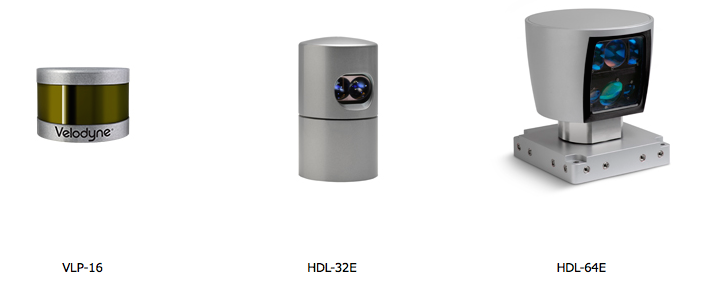
\includegraphics[width=0.8\columnwidth]{figs/3dsensors/velodyne}
   \caption{Velodyne Models}
   \label{fig::velodyne_models}
\end{figure}

\paragraph{Forecast 3D Laser System}


O sensor Forecast 3D consiste em um senor 2D laser da SICK, modelo LMS 151 ou
511, acoplado a uma unidade $pan-tilt$. O seu preço esta na faixa de U\$37k.


\begin{figure}[h!]
   \centering
   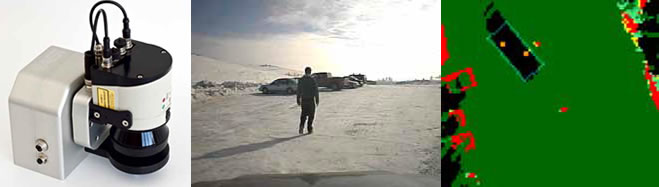
\includegraphics[width=0.8\columnwidth]{figs/3dsensors/forecast}
   \caption{Forecast 3D Laser System}
   \label{fig::forecast}
\end{figure}



\subsubsection{ToF Cameras}

As conhecidas como Time-of-Flight são dispositivos compostos por apenas uma
câmera, não necessitando de uma configuração stereo para triangularização de
imagens. Esse tipo de dispositivo utiliza uma fonte infra-vermelho interna e de
forma análoga aos dispositivos laser, calcula a distância a partir da diferença
de fase do sinal refletido. Entretanto, essa tecnologia possibilita o cálculo
simultâneo das distâncias de cada objeto na região iluminada pela fonte IR,
mesmo que com resoluções limitadas.

\paragraph{Sentis M100 / Argos 3D - P100}

\begin{itemize}
  \item Medidas de distância e vídeo em tons de cinza
  \item Resolução: 160 x 120 pixels
  \item 40 - 160 fps
  \item Alcance: $>$3m  (extensível até 10m indoor)
  \item Campo de Visão: $90^o$
  \item Tamanho: 75 x 57 x 26 mm
  \item Peso:
\end{itemize}

\begin{figure}[h!]
   \centering
   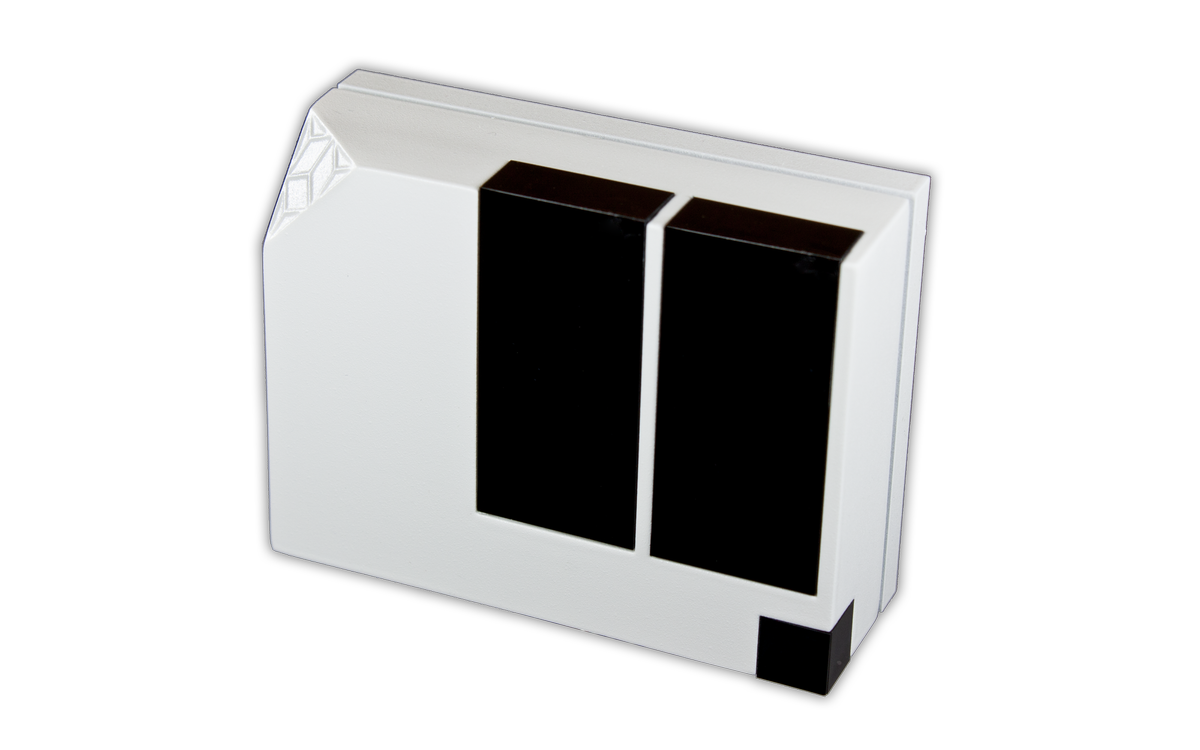
\includegraphics[width=0.8\columnwidth]{figs/3dsensors/argos3dp100}
   \caption{Sensor Argos 3D - P100}
   \label{fig::forecast}
\end{figure}


\subsection{Mesa Imaging SwissRanger SR4000}


\begin{itemize}
  \item Alcance para detecção: 0.1 - 10.0 m
  \item Alcance calibrado: 0.8 - 8.0 m
  \item Drift com a temperatura (T) - $\leq$ 1.5 mm/$^o$C (max.) - For 10$^o$C
  $\leq$ T $\leq$ 50$^o$C
  \item Tamanho: 65 x 65 x 76 mm
  \item Peso: 510 g
\end{itemize}

\begin{figure}[h!]
   \centering
   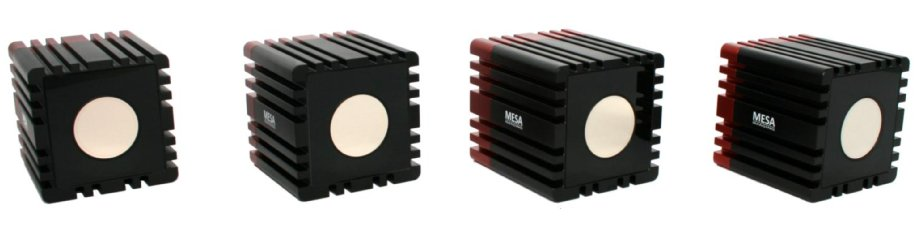
\includegraphics[width=0.8\columnwidth]{figs/3dsensors/mesa2}
   \caption{Mesa Imaging SwissRanger SR4000}
   \label{fig::mesa}
\end{figure}

%TODO exemplos dos sensores de ToF

Essa tecnologia tem como vantagem o tamanho relativamente compacto dos sensores,
não precisa de calibração extrínseca e também não é muito sensivel a iluminação
presente no ambiente, pois possui fonte de iluminação própria. Por não possuir
partes móveis, esse sensor possibilita a aquisição completa da imagem com altas
taxas de amotragem e, também, não há presença de efeito giroscópico como em
lasers rotativos.

%TODO Pros e cons

\subsubsection{Câmeras de Luz Estruturada}

Estes sensores constituem de uma fonte emissora de infra-vermelho e um receptor.
Um padrão é projetado na cena a ser reconstruida e a partir da distorção desse
padrão é possível o cálculo de distâncias. 

%TODO exemplos dos sensores de luz estruturada
%TODO Pros e cons

%TODO ELAEL - decidir se abre uma subseção d eaplicações ou coloca um exemplo de
% aplicação em cada componente - utilizar o seu material do SOTA em 3D sensors. 


